\documentclass[10pt,aspectratio=169]{beamer}

% Theme and colors
\usetheme{Madrid}
\usecolortheme{default}

\definecolor{darkblue}{RGB}{0,51,102}
\definecolor{lightblue}{RGB}{220,235,250}
\definecolor{accentred}{RGB}{180,30,30}
\definecolor{accentgreen}{RGB}{0,110,60}
\definecolor{midgray}{RGB}{100,100,100}

\setbeamercolor{structure}{fg=darkblue}
\setbeamercolor{title}{fg=white,bg=darkblue}
\setbeamercolor{frametitle}{fg=darkblue,bg=lightblue}
\setbeamercolor{block title}{fg=white,bg=darkblue}
\setbeamercolor{block body}{bg=lightblue}
\setbeamercolor{block title alerted}{fg=white,bg=accentred}
\setbeamercolor{block body alerted}{bg=red!5!white}
\setbeamercolor{block title example}{fg=white,bg=accentgreen}
\setbeamercolor{block body example}{bg=green!5!white}

% Smaller frametitle to avoid two-line titles
\setbeamerfont{frametitle}{size=\small,series=\bfseries}

\setbeamertemplate{navigation symbols}{}
\setbeamertemplate{footline}{%
  \hfill\insertframenumber/\inserttotalframenumber\hspace{0.5cm}\vspace{0.3cm}%
}

% Packages
\usepackage{amsmath,amssymb,amsthm}
\usepackage{graphicx}
\usepackage{tikz}
\usetikzlibrary{arrows.meta,positioning,calc,decorations.pathreplacing}
\usepackage{booktabs}
\usepackage{appendixnumberbeamer}

% Helper: colored icon circle
\newcommand{\iconcirc}[1]{%
  \tikz[baseline=-0.6ex]\node[circle,fill=darkblue,text=white,
    font=\bfseries\small,inner sep=3pt,minimum size=0.55cm]{#1};%
}

% Metadata
\title[BCG (2025)]{\textbf{Bottom-Up Markup Fluctuations}}
\subtitle{Burstein, Carvalho \& Grassi (QJE, 2025)}
\author{Tim K\"{u}hleis \\[0.5em]\small Empirical Industrial Organisation}
\date{April 2026}

\begin{document}

\begin{frame}
  \titlepage
\end{frame}

%% ============================================================
%% Slide 1: Introduction
%% ============================================================
\begin{frame}{Markup Cyclicality Remains an Open Empirical Puzzle}

\textbf{The puzzle:} The business cycle literature has established cyclicality for many variables --- unemployment countercyclical, investment procyclical. \textbf{Markups are a notable exception.}

\vspace{0.4em}
\begin{itemize}
  \item Bils \& Klenow (2018): markups \textbf{countercyclical} --- based on the entire U.S.\ economy
  \item Anderson, Rebelo \& Wong (2023): markups \textbf{acyclical} --- based on the U.S.\ retail sector
\end{itemize}

\vspace{0.4em}
\textbf{Why it matters:} Markups are the wedge between prices and marginal costs. Their cyclicality shapes how productivity shocks transmit to aggregate output and determines resource allocation over the cycle.

\vspace{0.4em}
\textbf{Key question:} Can the granularity lens reconcile these conflicting findings?

\vspace{0.4em}
\textbf{Burstein, Carvalho \& Grassi (QJE, 2025)} build the first granular model of markup fluctuations. Three core results:

\vspace{0.2em}
\begin{enumerate}
  \item The \textit{relative size} of the shocked firm determines its effect on sectoral and aggregate markups
  \item Short-sample correlations between markups and aggregate variables are highly unstable and can take either sign
  \item Fat tails imply that large firms' markup changes due to idiosyncratic shocks persist across aggregation levels
\end{enumerate}

\end{frame}

%% ============================================================
%% Slide 2: Building Blocks
%% ============================================================
\begin{frame}{Three Building Blocks Underpin the BCG Framework}

\vspace{0.1em}
\begin{columns}[T]

%% Column 1
\column{0.31\textwidth}

\begin{tikzpicture}
  \node[fill=darkblue, text=white, rounded corners,
        text width=\linewidth, align=center, inner sep=4pt]
    {\textbf{\footnotesize (1) Firm Size Distribution}\\[0.2em] {\scriptsize (Gabaix, 1999)}};
\end{tikzpicture}

\vspace{0.2em}
\begin{itemize}\footnotesize
  \item BCG model firm growth as a discretized random growth process with a lower \textbf{reflecting barrier}
  \vspace{0.2em}
  \item[\color{accentgreen}$\Rightarrow$] Gabaix (1999): resulting size distribution is \textbf{Pareto (fat-tailed)}, $\alpha \approx 1$
\end{itemize}

\vspace{0.5em}
{\scriptsize\color{midgray} Implemented as a C\'{o}rdoba (2008) Markov chain on a discrete productivity grid\par}

%% Column 2
\column{0.31\textwidth}

\begin{tikzpicture}
  \node[fill=darkblue, text=white, rounded corners,
        text width=\linewidth, align=center, inner sep=4pt]
    {\textbf{\footnotesize (2) Granularity}\\[0.2em] {\scriptsize (Gabaix, 2011)}};
\end{tikzpicture}

\vspace{0.2em}
\begin{itemize}\footnotesize
  \item Equal firms: $\sigma(\Delta Y) \sim 1/\sqrt{N}$ (CLT)
  \item Fat tails: large firms disproportionately influential
  \item Idiosyncratic shocks \textbf{do not diversify away}
  \vspace{0.2em}
  \item[\color{accentgreen}$\Rightarrow$] $\sigma(\Delta Y) \approx \sigma\cdot\sqrt{HHI}$
\end{itemize}

\vspace{0.5em}
{\scriptsize\color{midgray} Granular residual accounts for $\sim$1/3 of U.S.\ GDP volatility\par}

%% Column 3
\column{0.31\textwidth}

\begin{tikzpicture}
  \node[fill=darkblue, text=white, rounded corners,
        text width=\linewidth, align=center, inner sep=4pt]
    {\textbf{\footnotesize (3) Markups \& Market Share}\\[0.2em] {\scriptsize (Atkeson \& Burstein, 2008)}};
\end{tikzpicture}

\vspace{0.2em}
\begin{itemize}\footnotesize
  \item Nested CES: $\varepsilon$ within $>$ $\sigma$ across sectors
  \item Large firms internalize sector price effect $\Rightarrow$ less elastic demand
  \[
    \mu_i = \frac{\varepsilon}{\varepsilon-1}\!\left[1 - \frac{\varepsilon/\sigma-1}{\varepsilon-1}s_i\right]^{-1}
  \]
  \item[\color{accentgreen}$\Rightarrow$] Markup $\uparrow$ in $s_i$; pass-through \textbf{incomplete}
\end{itemize}

\end{columns}

\vspace{0.5em}
\begin{center}

\begin{tikzpicture}
  \draw[thick, darkblue, decorate, decoration={brace, amplitude=6pt, mirror}] (-6.25, 0) -- (6.25, 0);
  \draw[-Latex, thick, darkblue] (0, -6pt) -- (0, -0.4cm);
  \node[draw=darkblue, fill=lightblue, rounded corners, text width=12.5cm,
        align=center, inner sep=4pt, font=\footnotesize\bfseries, anchor=north] at (0, -0.4cm) {
    BCG (2025) combine all three to build the first granular model of markup fluctuations in the economy.
  };
\end{tikzpicture}
\end{center}

\end{frame}

%% ============================================================
%% Slide 3: Mechanisms
%% ============================================================
\begin{frame}{Firm Identity Determines Markup Responses at All Levels of Aggregation}

\vspace{-0.6em}
\begin{columns}[T]

\column{0.31\textwidth}
\begin{center}
  \iconcirc{F}\\[0.25em]
  {\color{darkblue}\small\textbf{Firm Level}}
\end{center}
\vspace{-1.2em}
\rule{\linewidth}{0.5pt}

\begin{itemize}\small
  \item {\footnotesize Productivity shock $\rightarrow$ $\downarrow$MC $\rightarrow$ output $\uparrow$ $\rightarrow$ share $\uparrow$ $\rightarrow$ markup $\uparrow$}
  \item Pass-through \textbf{incomplete}: part of productivity gain absorbed into markup
  \item[\color{accentgreen}$\Rightarrow$] Effect \textbf{larger for bigger firms}: pass-through decreasing in market share
\end{itemize}

\column{0.03\textwidth}
\vspace{0.6cm}
\begin{center}

\begin{tikzpicture}
  \draw[-Latex, ultra thick, darkblue!50] (0,0) -- (0.4,0);
\end{tikzpicture}
\end{center}

\column{0.31\textwidth}
\begin{center}
  \iconcirc{S}\\[0.25em]
  {\color{darkblue}\small\textbf{Sector Level}}
\end{center}
\vspace{-1.2em}
\rule{\linewidth}{0.5pt}

\begin{itemize}\small
  \item A shock to a \textbf{large} firm raises the sector markup; a shock to a \textbf{small} firm lowers it
  \item[\color{accentgreen}$\Rightarrow$] \textbf{Proposition 1:} whether $s_i$ exceeds a threshold $\bar{s}_k$ determines the sign of $\Delta\bar{\mu}_k$
  \item Firm \textbf{identity} determines the sign --- not shock size
\end{itemize}

\column{0.03\textwidth}
\vspace{0.6cm}
\begin{center}

\begin{tikzpicture}
  \draw[-Latex, ultra thick, darkblue!50] (0,0) -- (0.4,0);
\end{tikzpicture}
\end{center}

\column{0.31\textwidth}
\begin{center}
  \iconcirc{A}\\[0.25em]
  {\color{darkblue}\small\textbf{Aggregate Level}}
\end{center}
\vspace{-1.2em}
\rule{\linewidth}{0.5pt}

\begin{itemize}\small
  \item Fat-tailed size dist.\ $\Rightarrow$ large firms have disproportionate effect on aggregate markup (granularity argument)
  \item TFP shocks: shares unchanged, output rises $\Rightarrow$ markup flat
  \item[\color{accentred}$\Rightarrow$] \textbf{Aggregation paradox:}\\
        sector markups procyclical;\\
        aggregate near-acyclical;\\
        short samples: either sign
\end{itemize}

\end{columns}

\end{frame}

%% ============================================================
%% Slide 4: Monte Carlo
%% ============================================================
\begin{frame}{Monte Carlo Simulations Confirm All Three Mechanisms}

\vspace{0.1em}
\begin{center}
  \includegraphics[width=0.85\textwidth]{../01_Outputs/fig_combined.pdf}
\end{center}

\vspace{0.1em}
\begin{center}
{\footnotesize
\begin{tabular}{@{}cl@{\hspace{1.5em}}cl@{}}
  \textbf{A:} & Firm identity determines sign (Prop.\ 1) &
  \textbf{B\,\&\,C:} & Aggregation paradox; short samples volatile \\[0.1em]
  \textbf{D:} & Fatter tails $\Rightarrow$ slower diversification &
  & \\
\end{tabular}}
\end{center}

\end{frame}

%% ============================================================
%% Slide 5: Discussion and Conclusion
%% ============================================================
\begin{frame}{Takeaway}

\vspace{1.8cm}
\begin{center}
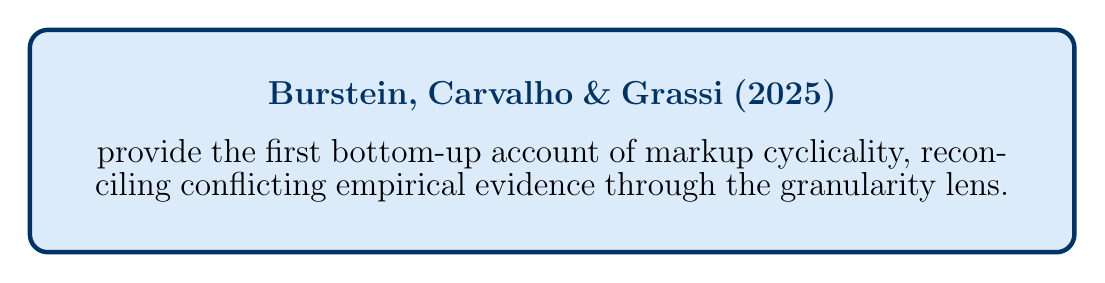
\begin{tikzpicture}
  \node[draw=darkblue, ultra thick, fill=lightblue, rounded corners=1.5ex,
        text width=12cm, align=center, inner sep=18pt] {
    {\large\color{darkblue}\textbf{Burstein, Carvalho \& Grassi (2025)}}\\[0.9em]
    {\large provide the first bottom-up account of markup cyclicality,
    reconciling conflicting empirical evidence through the granularity lens.}
  };
\end{tikzpicture}

\vspace{1.2cm}
{\normalsize\color{midgray} Thank you}
\end{center}

\end{frame}

\end{document}
